\section*{1.}
As seen from Figure~\ref{fig:inverse} there are no visual artifacts introduced, so the images should be the same. The blockproc source code can be found in Listing~\ref{lst:blockproc}. The image is opened in Listing~\ref{lst:open}, and the transformations are executed in Listings~\ref{lst:transdct} and~\ref{lst:transdft}.

\begin{figure}[H]
	\centering
	\begin{subfigure}[t]{0.5\textwidth}
		\centering
		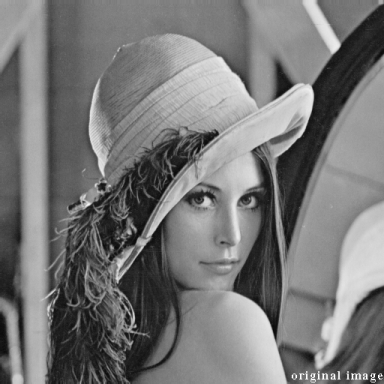
\includegraphics[width=0.9\textwidth]{transform-dct}
		\caption{DCT transformed}
	\end{subfigure}%
	~
	\begin{subfigure}[t]{0.5\textwidth}
		\centering
		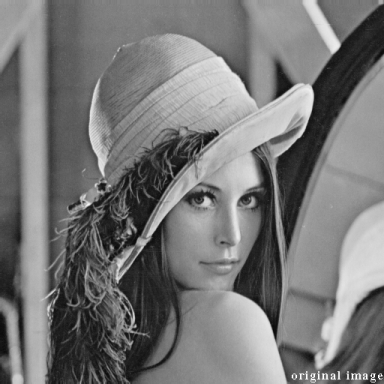
\includegraphics[width=0.9\textwidth]{transform-dft}
		\caption{DFT transformed}
	\end{subfigure}%
	\caption{DCT and DFT inversed Lena images}
	\label{fig:inverse}
\end{figure}

\lstinputlisting[
  language=Python,
  firstline=11,
  lastline=24,
  label={lst:blockproc},
  caption={blockproc function definition}]
  {code.py}

\lstinputlisting[
  language=Python,
  firstline=132,
  lastline=133,
  label={lst:open},
  caption={Opening image}]
  {code.py}

\lstinputlisting[
  language=Python,
  firstline=137,
  lastline=141,
  label={lst:transdct},
  caption={DCT transfomration}]
  {code.py}

\lstinputlisting[
  language=Python,
  firstline=145,
  lastline=149,
  label={lst:transdft},
  caption={DFT transformation}]
  {code.py}

\section*{2.}
\(A = \displaystyle\sum_{i = 1}^{mn} (A, \phi_i) \phi_i\)
\\
\\
\\
\(\hat{A} = \displaystyle\sum_{i \in I_n} (A, \phi_i) \phi_i\)
\\
\\
\\
\(D(c) = \frac{\norm{A - \hat{A}}^2}{\norm{A}^2}\)
\\
\\
\\
Thus, \(D(c) = \frac{\norm{\displaystyle\sum_{i = 1}^{mn} (A, \phi_i) \phi_i - \displaystyle\sum_{i \in I_n} (A, \phi_i) \phi_i}^2}{\norm{\displaystyle\sum_{i = 1}^{mn} (A, \phi_i) \phi_i}^2}\)
\\
\\
\\
The final value depends on how close the numerator in the formula above is to the denominator.
If the numerator is the same as the denominator, the distortion will be 1.
If it is 0, the distortion will be 0.
The value of the numerator depends on how much difference there is between \(A\) and \(\hat{A}\).
If they are the same, the numerator will be 0, and thus the distortion will be 0.
The larger the difference is, the higher the numerator will be, and the larger the distortion will be.
If there is no data left in \(\hat{A}\), the numerator will be \(A\) and the distortion will be 1.

Because of this, if low amplitudes are selected for \(I_N\), \(\hat{A}\) will be low, and the difference will be high.
If high amplitudes are selected, \(\hat{A}\) will be high, and the difference will be low.
Thus, to lower the distortion, the highest amplitudes should be kept.

\section*{3.}
Figure~\ref{fig:compress} shows the DCT and DFT compressed images with an N of 8.
It is clear the the DFT version is worse because you can see the blocks much more clearly.
The images are compressed in Listings~\ref{lst:cmprdct} and~\ref{lst:cmprdft}.
The functions passed to blockproc are defined in Listing~\ref{lst:cmprfun}.
These functions use the compress function defined in Listing~\ref{lst:compress}.
Note that N from the task is named limit in the source code to not confuse it with the dimensions of the image/block.

\begin{figure}[H]
	\centering
	\begin{subfigure}[t]{0.5\textwidth}
		\centering
		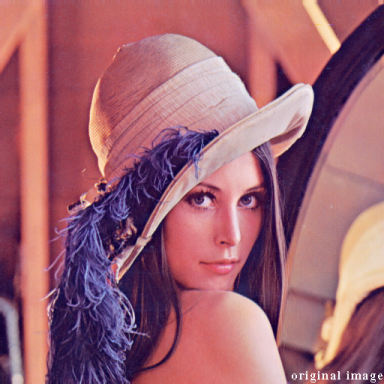
\includegraphics[width=0.9\textwidth]{lena}
		\caption{Original}
	\end{subfigure}%

	\centering
	\begin{subfigure}[t]{0.5\textwidth}
		\centering
		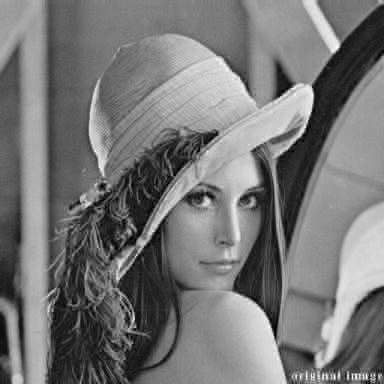
\includegraphics[width=0.9\textwidth]{compress-dct}
		\caption{DCT compressed}
	\end{subfigure}%
	~
	\begin{subfigure}[t]{0.5\textwidth}
		\centering
		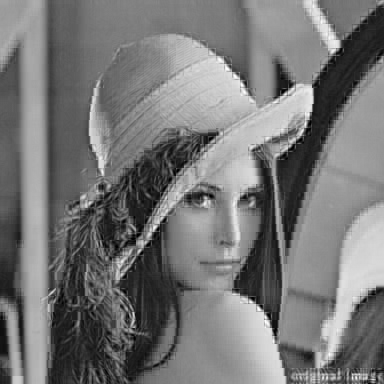
\includegraphics[width=0.9\textwidth]{compress-dft}
		\caption{DFT compressed}
	\end{subfigure}%
	\caption{DCT and DFT compressed Lena images}
	\label{fig:compress}
\end{figure}

\lstinputlisting[
  language=Python,
  firstline=153,
  lastline=157,
  label={lst:cmprdct},
  caption={DCT compression}]
  {code.py}

\lstinputlisting[
  language=Python,
  firstline=161,
  lastline=165,
  label={lst:cmprdft},
  caption={DFT compression}]
  {code.py}

\lstinputlisting[
  language=Python,
  firstline=43,
  lastline=48,
  label={lst:cmprfun},
  caption={DCT and DFT compression functions}]
  {code.py}

\lstinputlisting[
  language=Python,
  firstline=51,
  lastline=84,
  label={lst:compress},
  caption={compress function definition}]
  {code.py}

\section*{4.}
Figure~\ref{fig:distortion} shows the difference in distortion for using DCT and DFT with compression.
N=0 was not plotted since it will always be 1 (all data is lost) and make the rest of the plot too small to see any difference.
As you see from the source code, not all intervals were plotted for larger N.
This is because the compression algorithm written is very slow.
You can still clearly see the tendency in the graph.
You can clearly see from the plot that the compression with DCT performs better than DFT.
The difference in distortion gets lower with larger N.

Listing~\ref{lst:distortion} runs the plotting code.
It calls Listing~\ref{lst:distplot} to do the actual data plotting.
This function runs over all N (sample\_times) that should be plotted.
For each, Listing~\ref{lst:distcalc} is called to calculate the distortion between the synthesized and original image.

\begin{figure}[H]
  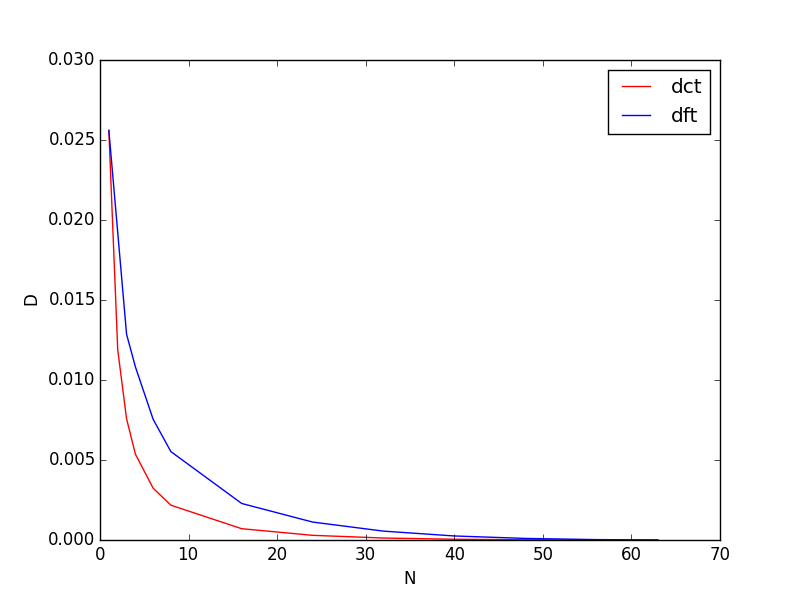
\includegraphics[width=\textwidth]{distortion}
  \caption{Plotted distortion of DCT vs DFT over N}
  \label{fig:distortion}
\end{figure}

\lstinputlisting[
  language=Python,
  firstline=168,
  lastline=182,
  label={lst:distortion},
  caption={Plot distortion of DCT and DFT compression}]
  {code.py}

\lstinputlisting[
  language=Python,
  firstline=98,
  lastline=107,
  label={lst:distplot},
  caption={Plot distortion}]
  {code.py}

\lstinputlisting[
  language=Python,
  firstline=87,
  lastline=95,
  label={lst:distcalc},
  caption={Calculate distortion}]
  {code.py}
